%%%% Paramétrage du TD %%%%
\def\xxactivite{ \ifprof \normalsize{Application 4 -- Corrigé } \else  \ifcolle Colle \else Application 4\fi \fi} % \normalsize \vspace{-.4cm}
\def\xxauteur{\textsl{Xavier Pessoles}}

\def\xxnumchapitre{Chapitre 1 \& 2 \vspace{.2cm}}
\def\xxchapitre{\hspace{.12cm} Chaînes de solides}



\def\xxcompetences{%
\vspace{-.5cm}
\footnotesize{
\textsl{%
\textbf{Savoirs et compétences :}\\
\vspace{-.2cm}
\begin{itemize}[label=\ding{112},font=\color{ocre}] 
\item \textit{Mod2.C34} : chaînes de solides;
\item \textit{Mod2.C34} : degré de mobilité du modèle;
\item \textit{Mod2.C34} : degré d’hyperstatisme du modèle;
%\item \textit{Mod2.C34.SF1} : déterminer les conditions géométriques associées à l’hyperstatisme;
%\item \textit{Mod2.C34} : résoudre le système associé à la fermeture cinématique et en déduire le degré de mobilité et d’hyperstatisme.
\end{itemize}}}}

\def\xxtitreexo{Appareil de mammographie « ISIS » (General Electric)}
\def\xxsourceexo{\hspace{.2cm} \footnotesize{Centrale MP 2004}}

\def\xxfigures{
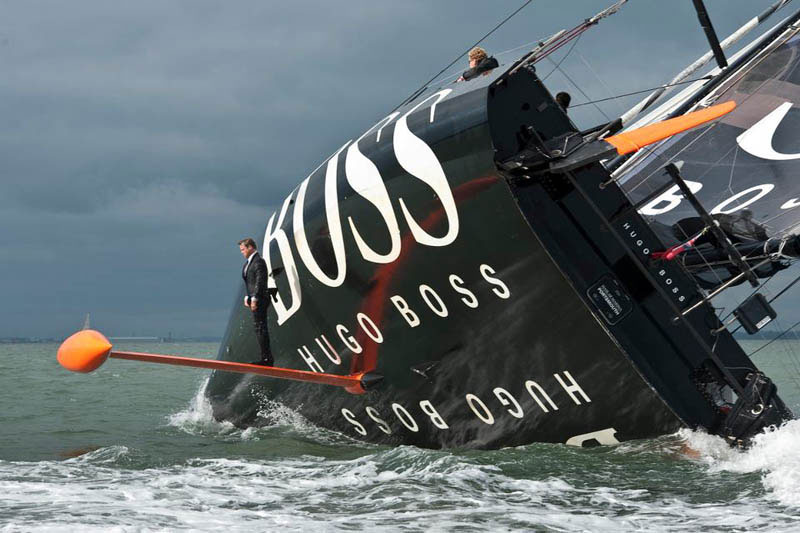
\includegraphics[width=.5\textwidth]{fig_00}
}%figues de la page de garde




\iflivret
\pagestyle{empty}


%%%%%%%% PAGE DE GARDE COURS
\ifcours
% ==== BANDEAU DES TITRES ==== 
\begin{tikzpicture}[remember picture,overlay]
\node at (current page.north west)
{\begin{tikzpicture}[remember picture,overlay]
\node[anchor=north west,inner sep=0pt] at (0,0) {\includegraphics[width=\paperwidth]{\thechapterimage}};
\draw[anchor=west] (-2cm,-8cm) node [line width=2pt,rounded corners=15pt,draw=ocre,fill=white,fill opacity=0.6,inner sep=40pt]{\strut\makebox[22cm]{}};
\draw[anchor=west] (1cm,-8cm) node {\huge\sffamily\bfseries\color{black} %
\begin{minipage}{1cm}
\rotatebox{90}{\LARGE\sffamily\textsc{\color{ocre}\textbf{\xxnumpartie}}}
\end{minipage} \hfill
\begin{minipage}[c]{14cm}
\begin{titrepartie}
\begin{flushright}
\renewcommand{\baselinestretch}{1.1} 
\Large\sffamily\textsc{\textbf{\xxpartie}}
\renewcommand{\baselinestretch}{1} 
\end{flushright}
\end{titrepartie}
\end{minipage} \hfill
\begin{minipage}[c]{3.5cm}
{\large\sffamily\textsc{\textbf{\color{ocre} \discipline}}}
\end{minipage} 
 };
\end{tikzpicture}};
\end{tikzpicture}
% ==== FIN BANDEAU DES TITRES ==== 


% ==== ONGLET 
\begin{tikzpicture}[overlay]
\node[shape=rectangle, 
      rounded corners = .25 cm,
	  draw= ocre,
	  line width=2pt, 
	  fill = ocre!10,
	  minimum width  = 2.5cm,
	  minimum height = 3cm,] at (18.3cm,0) {};
\node at (17.7cm,0) {\rotatebox{90}{\textbf{\Large\color{ocre}{\classe}}}};
%{};
\end{tikzpicture}
% ==== FIN ONGLET 


\vspace{3.5cm}

\begin{tikzpicture}[remember picture,overlay]
\draw[anchor=west] (-2cm,-6cm) node {\huge\sffamily\bfseries\color{black} %
\begin{minipage}{2cm}
\begin{center}
\LARGE\sffamily\textsc{\color{ocre}\textbf{\xxactivite}}
\end{center}
\end{minipage} \hfill
\begin{minipage}[c]{15cm}
\begin{titrechapitre}
\renewcommand{\baselinestretch}{1.1} 
\Large\sffamily\textsc{\textbf{\xxnumchapitre}}

\Large\sffamily\textsc{\textbf{\xxchapitre}}
\vspace{.5cm}

\renewcommand{\baselinestretch}{1} 
\normalsize\normalfont
\xxcompetences
\end{titrechapitre}
\end{minipage}  };
\end{tikzpicture}
\vfill

\begin{flushright}
\begin{minipage}[c]{.3\linewidth}
\begin{center}
\xxfigures
\end{center}
\end{minipage}\hfill
\begin{minipage}[c]{.6\linewidth}
\startcontents
%\printcontents{}{1}{}
\printcontents{}{1}{}
\end{minipage}
\end{flushright}

\begin{tikzpicture}[remember picture,overlay]
\draw[anchor=west] (4.5cm,-.7cm) node {
\begin{minipage}[c]{.2\linewidth}
\begin{flushright}

\includegraphics[width=2cm]{logoCC}
\end{flushright}
\end{minipage}
\begin{minipage}[c]{.2\linewidth}
\textsl{\xxauteur} \\
\textsl{\classe}
\end{minipage}
 };
\end{tikzpicture}

\newpage
\pagestyle{fancy}

%\newpage
%\pagestyle{fancy}

\else
\fi
%% FIN PAGE DE GARDE DES COURS

%%%%%%%% PAGE DE GARDE TD
\iftd
%\begin{tikzpicture}[remember picture,overlay]
%\node at (current page.north west)
%{\begin{tikzpicture}[remember picture,overlay]
%\draw[anchor=west] (-2cm,-3.25cm) node [line width=2pt,rounded corners=15pt,draw=ocre,fill=white,fill opacity=0.6,inner sep=40pt]{\strut\makebox[22cm]{}};
%\draw[anchor=west] (1cm,-3.25cm) node {\huge\sffamily\bfseries\color{black} %
%\begin{minipage}{1cm}
%\rotatebox{90}{\LARGE\sffamily\textsc{\color{ocre}\textbf{\xxnumpartie}}}
%\end{minipage} \hfill
%\begin{minipage}[c]{13.5cm}
%\begin{titrepartie}
%\begin{flushright}
%\renewcommand{\baselinestretch}{1.1} 
%\Large\sffamily\textsc{\textbf{\xxpartie}}
%\renewcommand{\baselinestretch}{1} 
%\end{flushright}
%\end{titrepartie}
%\end{minipage} \hfill
%\begin{minipage}[c]{3.5cm}
%{\large\sffamily\textsc{\textbf{\color{ocre} \discipline}}}
%\end{minipage} 
% };
%\end{tikzpicture}};
%\end{tikzpicture}

%%%%%%%%%% PAGE DE GARDE TD %%%%%%%%%%%%%%%
%\begin{tikzpicture}[overlay]
%\node[shape=rectangle, 
%      rounded corners = .25 cm,
%	  draw= ocre,
%	  line width=2pt, 
%	  fill = ocre!10,
%	  minimum width  = 2.5cm,
%	  minimum height = 2.5cm,] at (18.5cm,0) {};
%\node at (17.7cm,0) {\rotatebox{90}{\textbf{\Large\color{ocre}{\classe}}}};
%%{};
%\end{tikzpicture}

% PARTIE ET CHAPITRE
%\begin{tikzpicture}[remember picture,overlay]
%\draw[anchor=west] (-1cm,-2.1cm) node {\large\sffamily\bfseries\color{black} %
%\begin{minipage}[c]{15cm}
%\begin{flushleft}
%\xxnumchapitre \\
%\xxchapitre
%\end{flushleft}
%\end{minipage}  };
%\end{tikzpicture}

% BANDEAU EXO
\iflivret % SI LIVRET
\begin{tikzpicture}[remember picture,overlay]
\draw[anchor=west] (-2cm,-3.3cm) node {\huge\sffamily\bfseries\color{black} %
\begin{minipage}{5cm}
\begin{center}
\LARGE\sffamily\color{ocre}\textbf{\textsc{\xxactivite}}

\begin{center}
\xxfigures
\end{center}

\end{center}
\end{minipage} \hfill
\begin{minipage}[c]{12cm}
\begin{titrechapitre}
\renewcommand{\baselinestretch}{1.1} 
\large\sffamily\textbf{\textsc{\xxtitreexo}}

\small\sffamily{\textbf{\textit{\color{black!70}\xxsourceexo}}}
\vspace{.5cm}

\renewcommand{\baselinestretch}{1} 
\normalsize\normalfont
\xxcompetences
\end{titrechapitre}
\end{minipage}};
\end{tikzpicture}
\else % ELSE NOT LIVRET
\begin{tikzpicture}[remember picture,overlay]
\draw[anchor=west] (-2cm,-4.5cm) node {\huge\sffamily\bfseries\color{black} %
\begin{minipage}{5cm}
\begin{center}
\LARGE\sffamily\color{ocre}\textbf{\textsc{\xxactivite}}

\begin{center}
\xxfigures
\end{center}

\end{center}
\end{minipage} \hfill
\begin{minipage}[c]{12cm}
\begin{titrechapitre}
\renewcommand{\baselinestretch}{1.1} 
\large\sffamily\textbf{\textsc{\xxtitreexo}}

\small\sffamily{\textbf{\textit{\color{black!70}\xxsourceexo}}}
\vspace{.5cm}

\renewcommand{\baselinestretch}{1} 
\normalsize\normalfont
\xxcompetences
\end{titrechapitre}
\end{minipage}};
\end{tikzpicture}

\fi

\else   % FIN IF TD
\fi


%%%%%%%% PAGE DE GARDE FICHE
\iffiche
\begin{tikzpicture}[remember picture,overlay]
\node at (current page.north west)
{\begin{tikzpicture}[remember picture,overlay]
\draw[anchor=west] (-2cm,-2.25cm) node [line width=2pt,rounded corners=15pt,draw=ocre,fill=white,fill opacity=0.6,inner sep=40pt]{\strut\makebox[22cm]{}};
\draw[anchor=west] (1cm,-2.25cm) node {\huge\sffamily\bfseries\color{black} %
\begin{minipage}{1cm}
\rotatebox{90}{\LARGE\sffamily\textsc{\color{ocre}\textbf{\xxnumpartie}}}
\end{minipage} \hfill
\begin{minipage}[c]{14cm}
\begin{titrepartie}
\begin{flushright}
\renewcommand{\baselinestretch}{1.1} 
\large\sffamily\textsc{\textbf{\xxpartie} \\} 

\vspace{.2cm}

\normalsize\sffamily\textsc{\textbf{\xxnumchapitre -- \xxchapitre}}
\renewcommand{\baselinestretch}{1} 
\end{flushright}
\end{titrepartie}
\end{minipage} \hfill
\begin{minipage}[c]{3.5cm}
{\large\sffamily\textsc{\textbf{\color{ocre} \discipline}}}
\end{minipage} 
 };
\end{tikzpicture}};
\end{tikzpicture}

\iflivret
\begin{tikzpicture}[overlay]
\node[shape=rectangle, 
      rounded corners = .25 cm,
	  draw= ocre,
	  line width=2pt, 
	  fill = ocre!10,
	  minimum width  = 2.5cm,
	  minimum height = 2.5cm,] at (18.5cm,1.1cm) {};
\node at (17.9cm,1.1cm) {\rotatebox{90}{\textsf{\textbf{\large\color{ocre}{\classe}}}}};
%{};
\end{tikzpicture}
\else
\begin{tikzpicture}[overlay]
\node[shape=rectangle, 
      rounded corners = .25 cm,
	  draw= ocre,
	  line width=2pt, 
	  fill = ocre!10,
	  minimum width  = 2.5cm,
%	  minimum height = 2.5cm,] at (18.5cm,1.1cm) {};
	  minimum height = 2.5cm,] at (18.6cm,0cm) {};
\node at (18cm,0cm) {\rotatebox{90}{\textsf{\textbf{\large\color{ocre}{\classe}}}}};
%{};
\end{tikzpicture}

\fi

\else
\fi



\else
\pagestyle{empty}


%%%%%%%% PAGE DE GARDE COURS
\ifcours
% ==== BANDEAU DES TITRES ==== 
\begin{tikzpicture}[remember picture,overlay]
\node at (current page.north west)
{\begin{tikzpicture}[remember picture,overlay]
\node[anchor=north west,inner sep=0pt] at (0,0) {\includegraphics[width=\paperwidth]{\thechapterimage}};
\draw[anchor=west] (-2cm,-8cm) node [line width=2pt,rounded corners=15pt,draw=ocre,fill=white,fill opacity=0.6,inner sep=40pt]{\strut\makebox[22cm]{}};
\draw[anchor=west] (1cm,-8cm) node {\huge\sffamily\bfseries\color{black} %
\begin{minipage}{1cm}
\rotatebox{90}{\LARGE\sffamily\textsc{\color{ocre}\textbf{\xxnumpartie}}}
\end{minipage} \hfill
\begin{minipage}[c]{14cm}
\begin{titrepartie}
\begin{flushright}
\renewcommand{\baselinestretch}{1.1} 
\Large\sffamily\textsc{\textbf{\xxpartie}}
\renewcommand{\baselinestretch}{1} 
\end{flushright}
\end{titrepartie}
\end{minipage} \hfill
\begin{minipage}[c]{3.5cm}
{\large\sffamily\textsc{\textbf{\color{ocre} \discipline}}}
\end{minipage} 
 };
\end{tikzpicture}};
\end{tikzpicture}
% ==== FIN BANDEAU DES TITRES ==== 


% ==== ONGLET 
\begin{tikzpicture}[overlay]
\node[shape=rectangle, 
      rounded corners = .25 cm,
	  draw= ocre,
	  line width=2pt, 
	  fill = ocre!10,
	  minimum width  = 2.5cm,
	  minimum height = 3cm,] at (18.3cm,0) {};
\node at (17.7cm,0) {\rotatebox{90}{\textbf{\Large\color{ocre}{\classe}}}};
%{};
\end{tikzpicture}
% ==== FIN ONGLET 


\vspace{3.5cm}

\begin{tikzpicture}[remember picture,overlay]
\draw[anchor=west] (-2cm,-6cm) node {\huge\sffamily\bfseries\color{black} %
\begin{minipage}{2cm}
\begin{center}
\LARGE\sffamily\textsc{\color{ocre}\textbf{\xxactivite}}
\end{center}
\end{minipage} \hfill
\begin{minipage}[c]{15cm}
\begin{titrechapitre}
\renewcommand{\baselinestretch}{1.1} 
\Large\sffamily\textsc{\textbf{\xxnumchapitre}}

\Large\sffamily\textsc{\textbf{\xxchapitre}}
\vspace{.5cm}

\renewcommand{\baselinestretch}{1} 
\normalsize\normalfont
\xxcompetences
\end{titrechapitre}
\end{minipage}  };
\end{tikzpicture}
\vfill

\begin{flushright}
\begin{minipage}[c]{.3\linewidth}
\begin{center}
\xxfigures
\end{center}
\end{minipage}\hfill
\begin{minipage}[c]{.6\linewidth}
\startcontents
%\printcontents{}{1}{}
\printcontents{}{1}{}
\end{minipage}
\end{flushright}

\begin{tikzpicture}[remember picture,overlay]
\draw[anchor=west] (4.5cm,-.7cm) node {
\begin{minipage}[c]{.2\linewidth}
\begin{flushright}

\includegraphics[width=2cm]{logoCC}
\end{flushright}
\end{minipage}
\begin{minipage}[c]{.2\linewidth}
\textsl{\xxauteur} \\
\textsl{\classe}
\end{minipage}
 };
\end{tikzpicture}

\newpage
\pagestyle{fancy}

%\newpage
%\pagestyle{fancy}

\else
\fi
%% FIN PAGE DE GARDE DES COURS

%%%%%%%% PAGE DE GARDE TD
\iftd
%\begin{tikzpicture}[remember picture,overlay]
%\node at (current page.north west)
%{\begin{tikzpicture}[remember picture,overlay]
%\draw[anchor=west] (-2cm,-3.25cm) node [line width=2pt,rounded corners=15pt,draw=ocre,fill=white,fill opacity=0.6,inner sep=40pt]{\strut\makebox[22cm]{}};
%\draw[anchor=west] (1cm,-3.25cm) node {\huge\sffamily\bfseries\color{black} %
%\begin{minipage}{1cm}
%\rotatebox{90}{\LARGE\sffamily\textsc{\color{ocre}\textbf{\xxnumpartie}}}
%\end{minipage} \hfill
%\begin{minipage}[c]{13.5cm}
%\begin{titrepartie}
%\begin{flushright}
%\renewcommand{\baselinestretch}{1.1} 
%\Large\sffamily\textsc{\textbf{\xxpartie}}
%\renewcommand{\baselinestretch}{1} 
%\end{flushright}
%\end{titrepartie}
%\end{minipage} \hfill
%\begin{minipage}[c]{3.5cm}
%{\large\sffamily\textsc{\textbf{\color{ocre} \discipline}}}
%\end{minipage} 
% };
%\end{tikzpicture}};
%\end{tikzpicture}

%%%%%%%%%% PAGE DE GARDE TD %%%%%%%%%%%%%%%
%\begin{tikzpicture}[overlay]
%\node[shape=rectangle, 
%      rounded corners = .25 cm,
%	  draw= ocre,
%	  line width=2pt, 
%	  fill = ocre!10,
%	  minimum width  = 2.5cm,
%	  minimum height = 2.5cm,] at (18.5cm,0) {};
%\node at (17.7cm,0) {\rotatebox{90}{\textbf{\Large\color{ocre}{\classe}}}};
%%{};
%\end{tikzpicture}

% PARTIE ET CHAPITRE
%\begin{tikzpicture}[remember picture,overlay]
%\draw[anchor=west] (-1cm,-2.1cm) node {\large\sffamily\bfseries\color{black} %
%\begin{minipage}[c]{15cm}
%\begin{flushleft}
%\xxnumchapitre \\
%\xxchapitre
%\end{flushleft}
%\end{minipage}  };
%\end{tikzpicture}

% BANDEAU EXO
\iflivret % SI LIVRET
\begin{tikzpicture}[remember picture,overlay]
\draw[anchor=west] (-2cm,-3.3cm) node {\huge\sffamily\bfseries\color{black} %
\begin{minipage}{5cm}
\begin{center}
\LARGE\sffamily\color{ocre}\textbf{\textsc{\xxactivite}}

\begin{center}
\xxfigures
\end{center}

\end{center}
\end{minipage} \hfill
\begin{minipage}[c]{12cm}
\begin{titrechapitre}
\renewcommand{\baselinestretch}{1.1} 
\large\sffamily\textbf{\textsc{\xxtitreexo}}

\small\sffamily{\textbf{\textit{\color{black!70}\xxsourceexo}}}
\vspace{.5cm}

\renewcommand{\baselinestretch}{1} 
\normalsize\normalfont
\xxcompetences
\end{titrechapitre}
\end{minipage}};
\end{tikzpicture}
\else % ELSE NOT LIVRET
\begin{tikzpicture}[remember picture,overlay]
\draw[anchor=west] (-2cm,-4.5cm) node {\huge\sffamily\bfseries\color{black} %
\begin{minipage}{5cm}
\begin{center}
\LARGE\sffamily\color{ocre}\textbf{\textsc{\xxactivite}}

\begin{center}
\xxfigures
\end{center}

\end{center}
\end{minipage} \hfill
\begin{minipage}[c]{12cm}
\begin{titrechapitre}
\renewcommand{\baselinestretch}{1.1} 
\large\sffamily\textbf{\textsc{\xxtitreexo}}

\small\sffamily{\textbf{\textit{\color{black!70}\xxsourceexo}}}
\vspace{.5cm}

\renewcommand{\baselinestretch}{1} 
\normalsize\normalfont
\xxcompetences
\end{titrechapitre}
\end{minipage}};
\end{tikzpicture}

\fi

\else   % FIN IF TD
\fi


%%%%%%%% PAGE DE GARDE FICHE
\iffiche
\begin{tikzpicture}[remember picture,overlay]
\node at (current page.north west)
{\begin{tikzpicture}[remember picture,overlay]
\draw[anchor=west] (-2cm,-2.25cm) node [line width=2pt,rounded corners=15pt,draw=ocre,fill=white,fill opacity=0.6,inner sep=40pt]{\strut\makebox[22cm]{}};
\draw[anchor=west] (1cm,-2.25cm) node {\huge\sffamily\bfseries\color{black} %
\begin{minipage}{1cm}
\rotatebox{90}{\LARGE\sffamily\textsc{\color{ocre}\textbf{\xxnumpartie}}}
\end{minipage} \hfill
\begin{minipage}[c]{14cm}
\begin{titrepartie}
\begin{flushright}
\renewcommand{\baselinestretch}{1.1} 
\large\sffamily\textsc{\textbf{\xxpartie} \\} 

\vspace{.2cm}

\normalsize\sffamily\textsc{\textbf{\xxnumchapitre -- \xxchapitre}}
\renewcommand{\baselinestretch}{1} 
\end{flushright}
\end{titrepartie}
\end{minipage} \hfill
\begin{minipage}[c]{3.5cm}
{\large\sffamily\textsc{\textbf{\color{ocre} \discipline}}}
\end{minipage} 
 };
\end{tikzpicture}};
\end{tikzpicture}

\iflivret
\begin{tikzpicture}[overlay]
\node[shape=rectangle, 
      rounded corners = .25 cm,
	  draw= ocre,
	  line width=2pt, 
	  fill = ocre!10,
	  minimum width  = 2.5cm,
	  minimum height = 2.5cm,] at (18.5cm,1.1cm) {};
\node at (17.9cm,1.1cm) {\rotatebox{90}{\textsf{\textbf{\large\color{ocre}{\classe}}}}};
%{};
\end{tikzpicture}
\else
\begin{tikzpicture}[overlay]
\node[shape=rectangle, 
      rounded corners = .25 cm,
	  draw= ocre,
	  line width=2pt, 
	  fill = ocre!10,
	  minimum width  = 2.5cm,
%	  minimum height = 2.5cm,] at (18.5cm,1.1cm) {};
	  minimum height = 2.5cm,] at (18.6cm,0cm) {};
\node at (18cm,0cm) {\rotatebox{90}{\textsf{\textbf{\large\color{ocre}{\classe}}}}};
%{};
\end{tikzpicture}

\fi

\else
\fi



\fi
\setlength{\columnseprule}{.1pt}

\pagestyle{fancy}
\thispagestyle{plain}

\ifprof
\vspace{5cm}
\else
\vspace{5cm}
\fi

\def\columnseprulecolor{\color{ocre}}
\setlength{\columnseprule}{0.4pt} 

%%%%%%%%%%%%%%%%%%%%%%%

\setcounter{exo}{0}



%\ifprof
%\else
\begin{multicols}{2}
%\fi


\section*{Mise en situation}



Le mammographe est utilisée pour rechercher la présence d’une tumeur dans un sein. Il est constitué des éléments génériques suivants.

\begin{center}
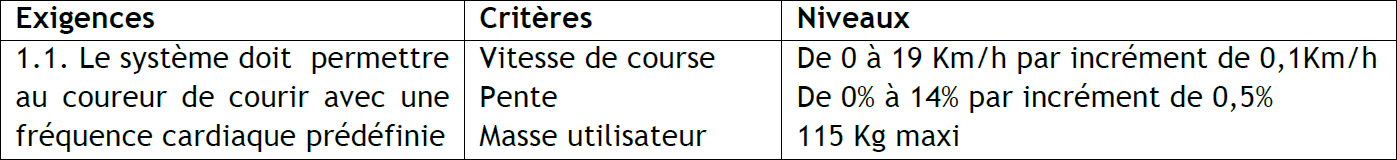
\includegraphics[width=\linewidth]{fig_02}
%\textit{}
\end{center}


Un ascenseur en liaison glissière de direction verticale par rapport à la partie fixe du mammographe (bâti). Cette mobilité permet d’adapter le mammographe à la taille de la patiente. L’ascenseur supporte les éléments suivants : la « tête RX » qui permet d’émettre les rayons X et un collimateur qui permet de contrôler le faisceau afin d’optimiser le cliché. Le réglage angulaire de la tête RX est réalisé par un pivotement autour de l’axe de rotation du mammographe.
La tête RX est donc en liaison pivot par rapport à l’ascenseur.


Le « bucky » sert de surface d’appui au sein et de support au film ou au capteur
d’images. %Il peut également recevoir le stéréotix permettant de réaliser une biopsie (prélèvement au niveau de la tumeur). 
Le réglage angulaire du
bucky est réalisé par un pivotement autour de l’axe de rotation du mammographe.
Le bucky est en liaison pivot par rapport à l’ascenseur.

La « plaque de pression » permet de comprimer le sein et de le maintenir en
position afin d’avoir une meilleure qualité de l’image. Elle fait l’objet d’une
liaison glissière par rapport au bucky.
À noter que les réglages angulaires des deux liaisons
pivots sont indépendants. On peut, par exemple, faire
tourner la tête sans faire tourner le bucky.
%
%Deux types d’examens radiologiques existent :
%\begin{itemize}
%\item le « screening » consiste en la prise de plusieurs clichés du sein suivant différents points de vue indépendants.
%Cet examen est 
%%C’est le premier examen radiologique effectué sur un sein. En particulier, c’est la procédure 
%utilisé lors des campagnes de dépistage systématique. En cas de diagnostic positif, l’examen de stéréatoxie peut être envisagé;
%\item la « stéréotaxie » consiste également en la prise de plusieurs clichés mais sans modifier le positionnement
%du sein sur le mammographe ni sa mise en pression. Les différentes vues 2D ainsi obtenues
%permettent d’identifier en 3D le positionnement précis de la tumeur. Les coordonnées de la tumeur sont
%alors communiquées au « stéréotix » afin de réaliser la biopsie avec précision.
%\end{itemize}

%%La chaîne image permet l’acquisition d’images numériques. Cette évolution technologique permet l’utilisation d’un logiciel capable de traiter l’image afin d’aider le radiologue dans la recherche des tumeurs de petites dimensions.

%
%\begin{center}
%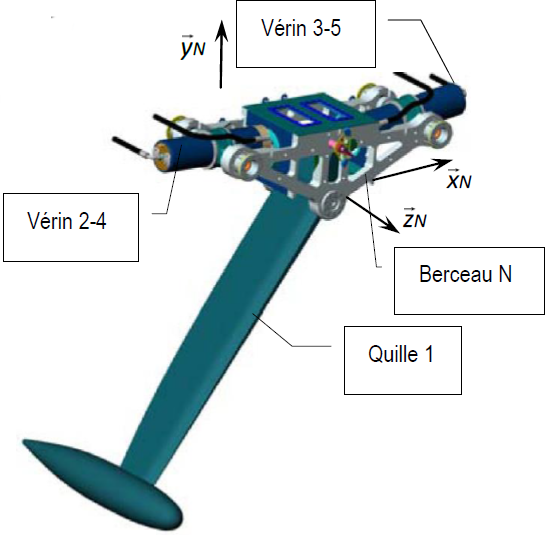
\includegraphics[width=.3\linewidth]{fig_03}
%\hspace{1cm}
%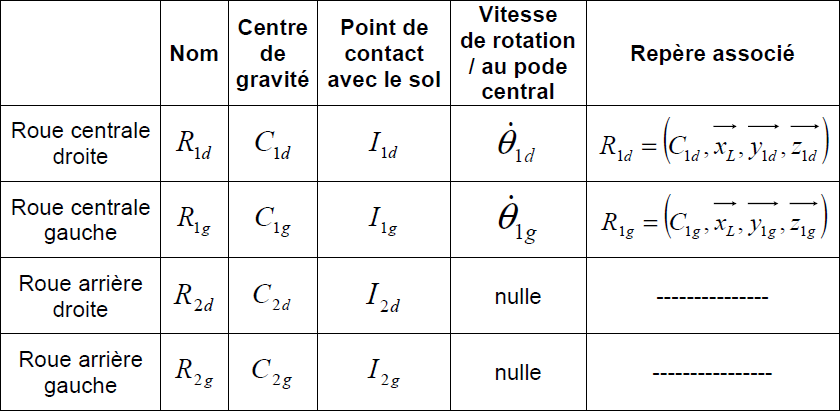
\includegraphics[width=.3\linewidth]{fig_04}
%%\textit{}
%\end{center}


\ifprof
\else
\begin{center}
%\includegraphics[width=\linewidth]{fig_00a}
%\textit{}
\end{center}
\fi

%\section*{Étude de l’architecture du mammographe ISIS}
%
%\begin{obj}
%L’objectif de cette étude est l’identification de la structure cinématique du mammographe.
%\end{obj}
%
%On peut hiérarchiser les fonctions décrivant un examen de type «~screening~».
%\begin{center}
%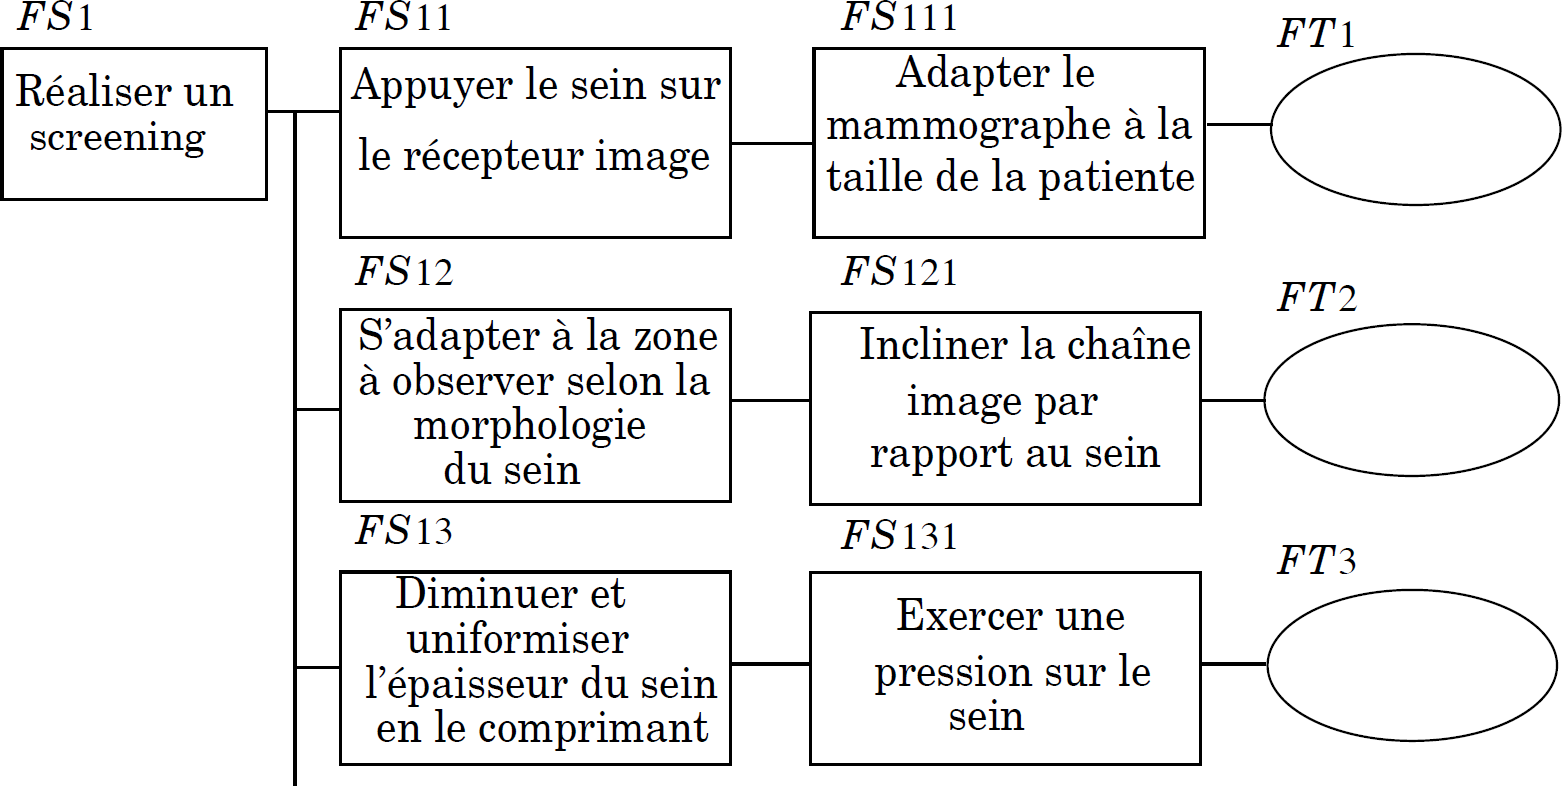
\includegraphics[width=\linewidth]{fig_05_bis}
%%\textit{}
%\end{center}
%
%\subparagraph{}\textit{Dans le cas d’un examen de type «~screening~», préciser le mouvement associé à la réalisation de chaque fonction technique FT1, FT2 et FT3. Pour chaque mouvement, indiquer si c’est une translation ou une rotation, la direction ou l’axe du mouvement, le (ou les solides) en mouvement relatif ainsi que le solide par rapport auquel il a lieu.}
%\ifprof
%\begin{corrige}~\\
%\end{corrige}
%\else
%\fi
%
%
%
%\subparagraph{}\textit{Par quel mouvement faut-il compléter la cinématique précédente pour
%que le mammographe permette également la réalisation d’un examen de type « stéréotaxie » ? Indiquer si c’est une
%translation ou une rotation, la direction ou l’axe du mouvement, le (ou les solides) en mouvement relatif ainsi que le
%solide par rapport auquel il a lieu.}
%\ifprof
%\begin{corrige}~\\
%\end{corrige}
%\else
%\fi
%
%
%
%
%\subparagraph{}\textit{Tracer le schéma cinématique en
%perspective du mammographe « ISIS »
%qui permet de réaliser les deux types
%d’examens.}
%\ifprof
%\begin{corrige}~\\
%\end{corrige}
%\else
%\fi
%
%\begin{center}
%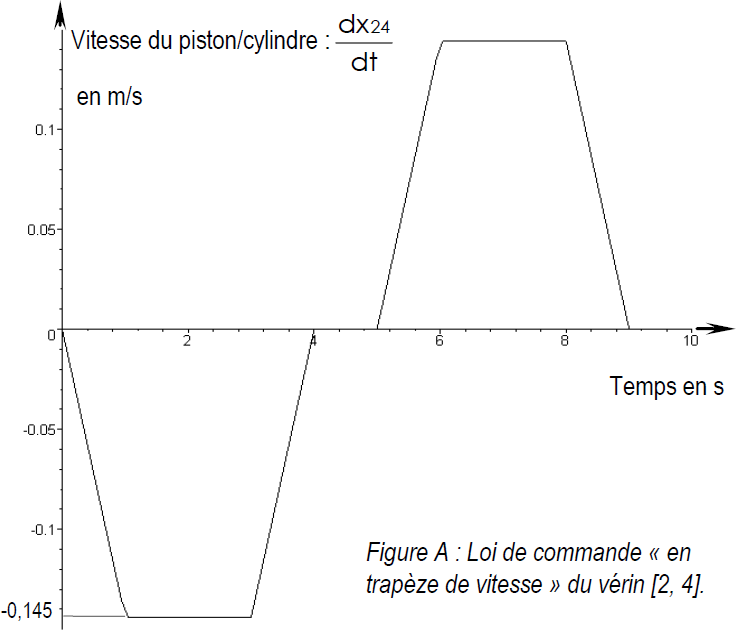
\includegraphics[width=.5\linewidth]{fig_06}
%%\textit{}
%\end{center}

\subsection*{Analyse de la fonction de service : « Adapter le
mammographe à la taille de la patiente » et de la fonction
technique associée : « faire monter et descendre
l’ascenseur »}

Le mammographe doit être adapté à la taille de la patiente en faisant monter
ou descendre l’ascenseur. La liaison glissière de l’ascenseur par rapport à la partie
fixe du mammographe est réalisée par un guidage sur deux barres parallèles
fixées sur le bâti. Le déplacement de l’ascenseur est obtenu à partir d’un moteur
électrique qui entraîne en rotation une vis. La rotation de la vis entraîne ensuite
l’écrou sur lequel est fixé l’ascenseur.
Un vérin à gaz permet d’assister le moteur lors de la montée de l’ascenseur par
l’intermédiaire d’une poulie montée à l’extrémité de la tige du vérin à gaz et
d’une courroie crantée. Une des extrémités de la courroie est fixée sur le bâti du
mammographe et l’autre extrémité est liée à l’ascenseur.

\begin{center}
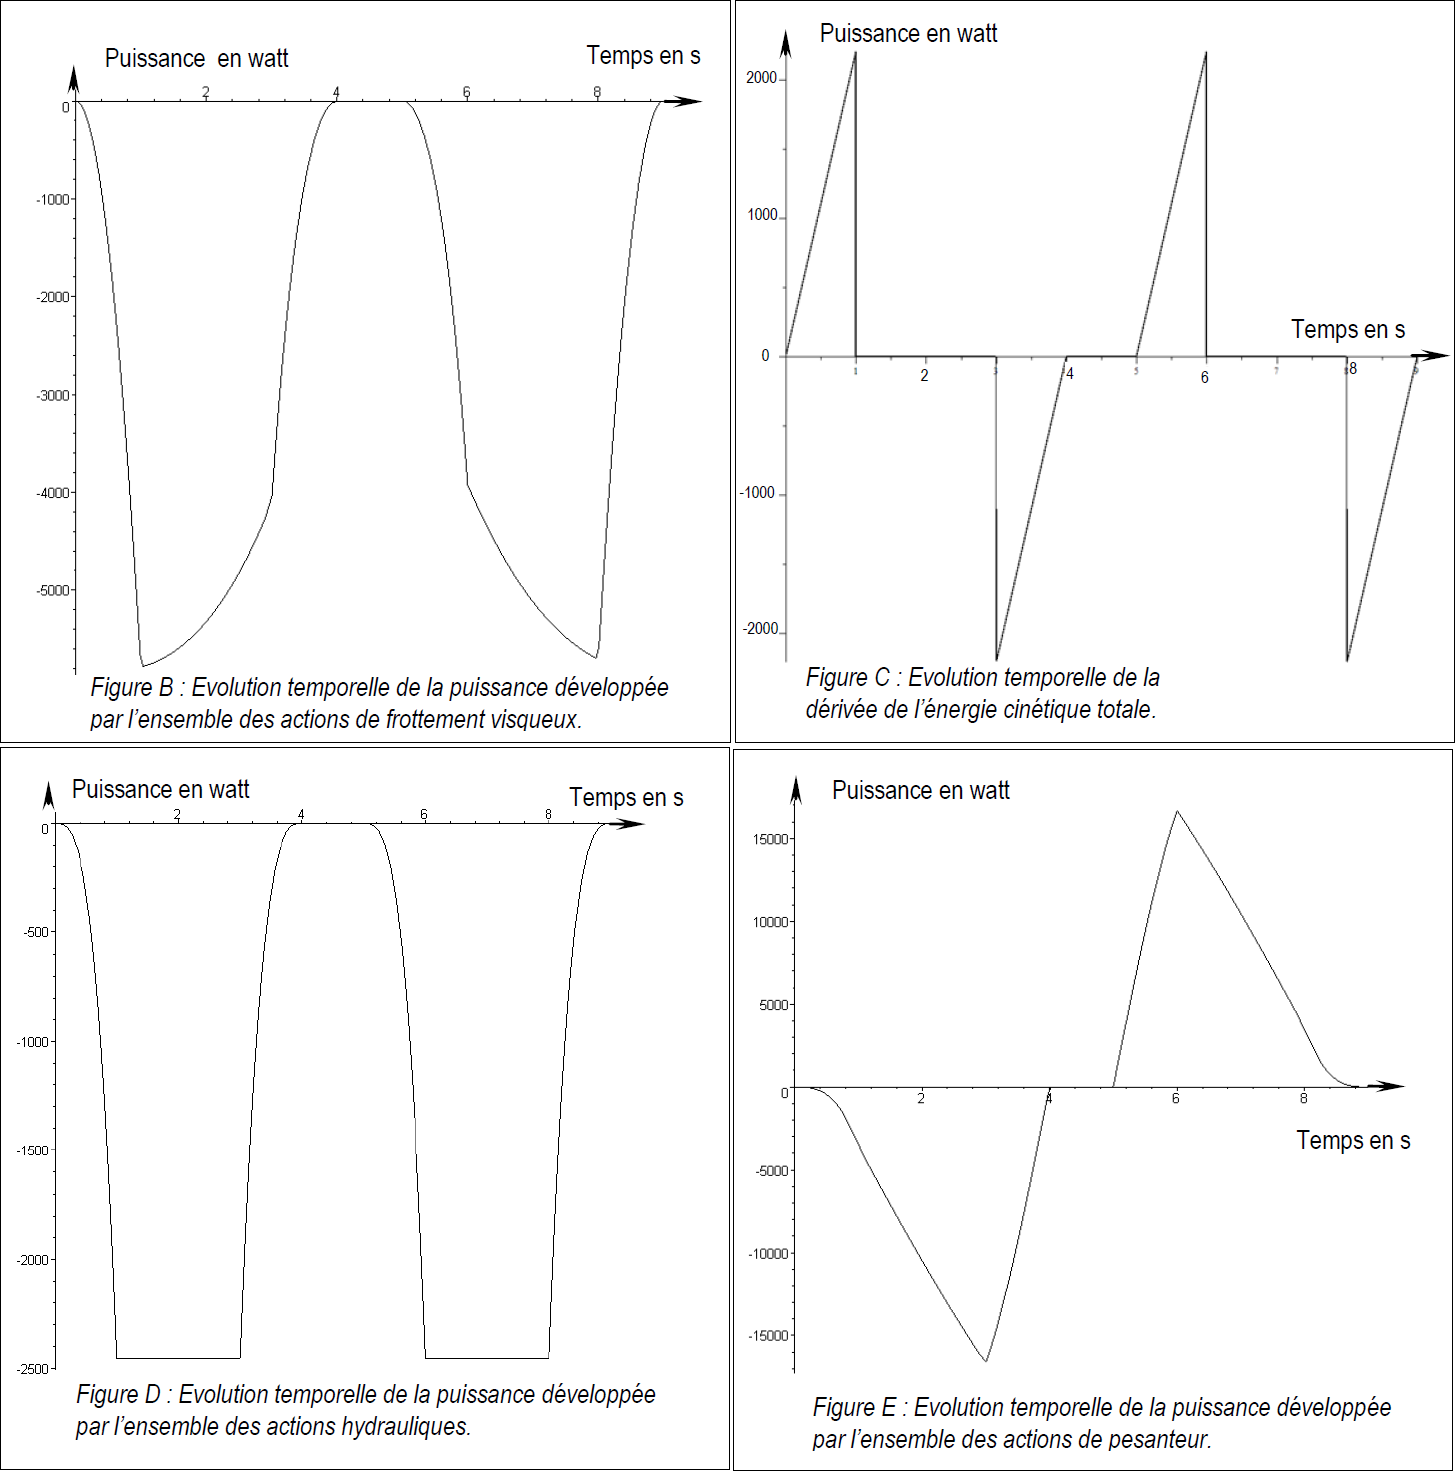
\includegraphics[width=.6\linewidth]{fig_07}
%\textit{}
\end{center}

\begin{center}
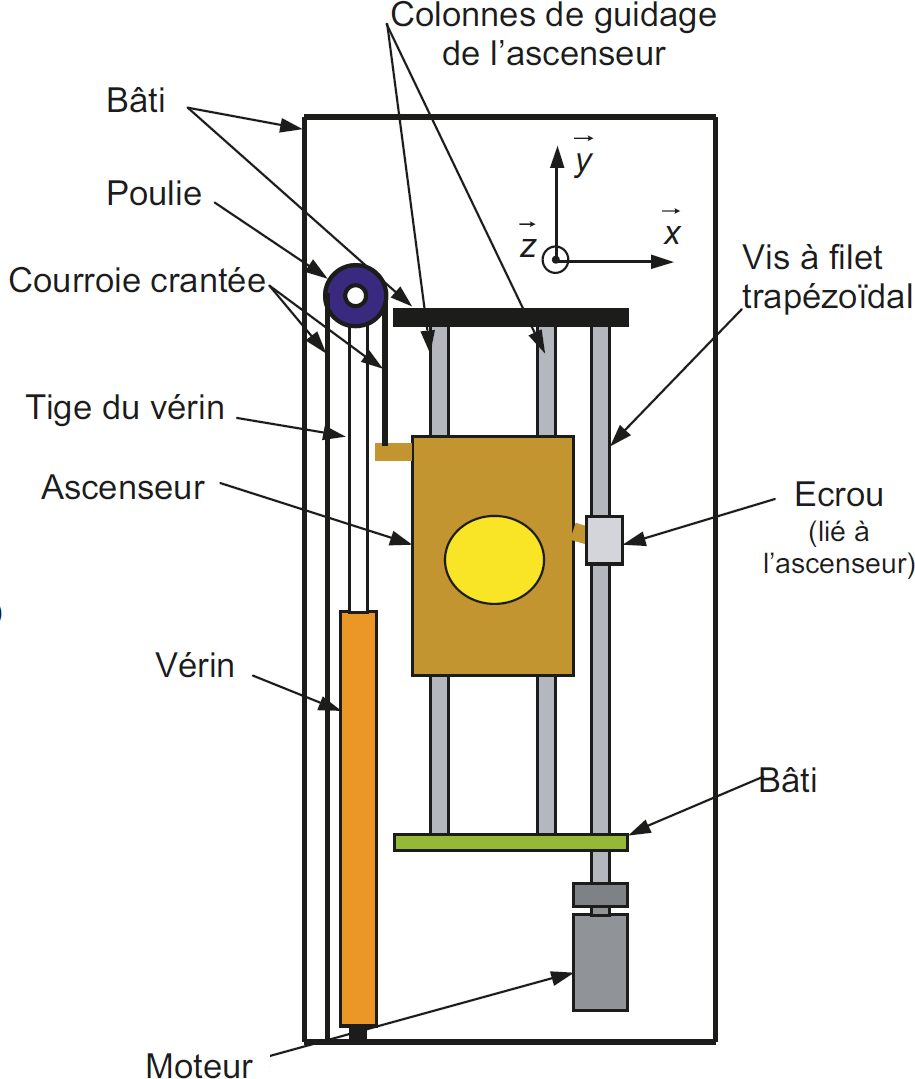
\includegraphics[width=.6\linewidth]{fig_08}
%\textit{}
\end{center}

\begin{center}
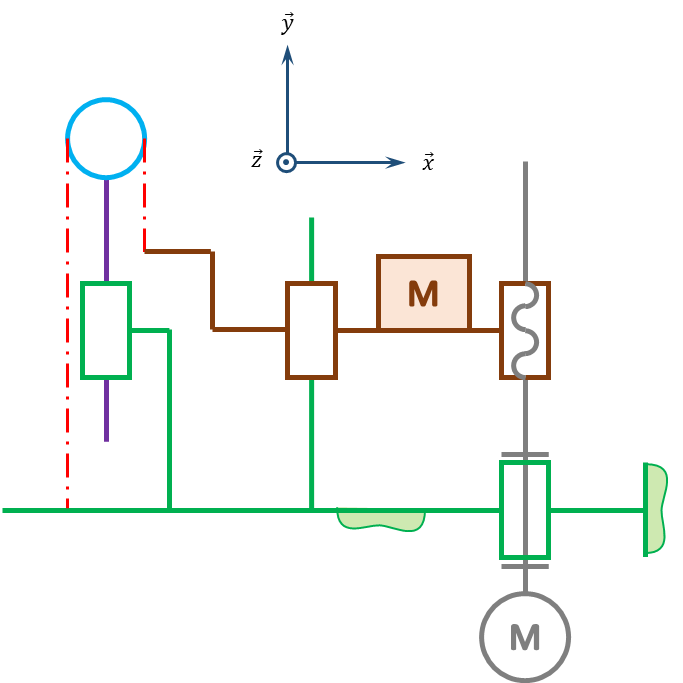
\includegraphics[width=\linewidth]{fig_10}
%\textit{}
\end{center}

%
%La figure précédente décrit la chaîne associée à la réalisation des fonctions techniques
%FT1 et FT2. Seuls les éléments intervenant dans FT1 sont repérés sur cette
%figure. Le schéma de principe de la chaîne associée à la
%réalisation de la fonction technique FT1 « Faire monter ou descendre
%l’ascenseur ».

\subsection*{Détermination de la motorisation}
\begin{obj}
L’objectif de cette étude est de valider la solution utilisant un vérin à gaz
pour assister le moteur, en la comparant à d’autres solutions
classiques : pas d’assistance, assistance à l’aide d’un contre-poids,
assistance à l’aide d’un ressort. Pour cela nous allons comparer les performances
minimales que doit avoir le moteur d’entraînement et vérifier
pour chaque cas la conformité au cahier des charges.
\end{obj}

\begin{center}
\begin{tabular}{|p{.6\linewidth}|p{.3\linewidth}|}
\hline
\multicolumn{2}{|c|}{Faire monter ou descendre l'ascenseur} \\
\hline
Critères & Niveaux \\
\hline
Ne pas stresser la patiente en déplaçant trop rapidement l’ascenseur : limiter la vitesse de
déplacement rapide & $V_R=\SI{0,15}{m.s^{-1}}$ \\ \hline
Ne pas blesser la patiente lors de l’approche du bucky : respecter une vitesse lente $V_L$ lors de
l’accostage & $V_L=\SI{0,02}{m.s^{-1}}$ \\ 
\hline
\end{tabular}
\end{center}


\begin{center}
%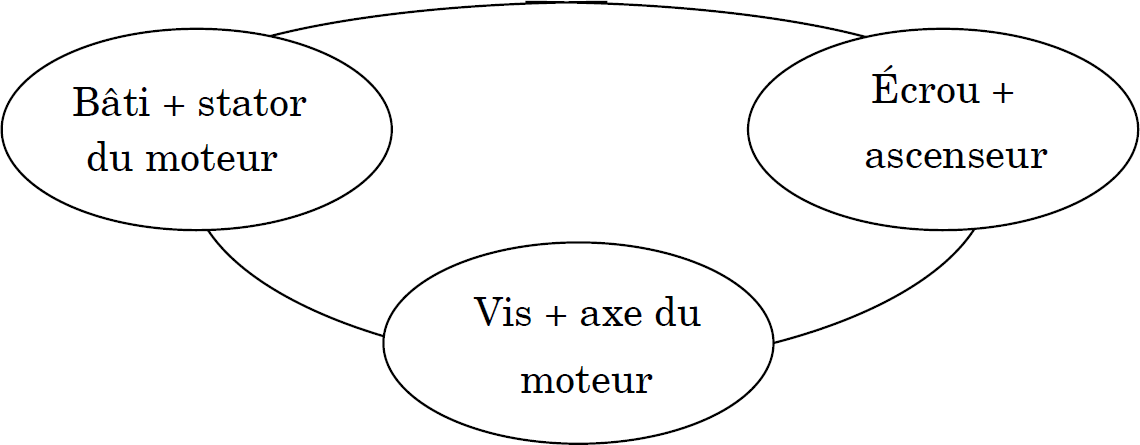
\includegraphics[width=.7\linewidth]{fig_09}
%\textit{}
\end{center}

\subparagraph{}\textit{Déterminer la vitesse de rotation du moteur $\omega$ en fonction de la vitesse de
déplacement $V$ de l’ascenseur. %Compléter alors, le bloc du schéma bloc dudocument réponse. 
En déduire la vitesse de rotation maximum $\omega_{\text{maxi}}$ que doit avoir le moteur, faire l’application numérique.}
\ifprof
\begin{corrige}~\\
On a $V=\omega \dfrac{p_v}{2\pi}$ et donc $\omega_{\text{maxi}} = V_R\dfrac{2\pi}{p_v}$.

Application numérique : $\omega_{\text{maxi}} = 0,15\dfrac{2\pi}{6\cdot 10^{-3}}=\SI{157}{rad.s^{-1}}$ $=\SI{1500}{tr.min^{-1}}$.
\end{corrige}
\else
\fi


\subparagraph{}\textit{}
\ifprof
\begin{corrige}~\\
\end{corrige}
\else
\fi



%\subparagraph{}\textit{}
%\ifprof
%\begin{corrige}~\\
%\end{corrige}
%\else
%\fi
%
%
%
%
%\subparagraph{}\textit{}
%\ifprof
%\begin{corrige}~\\
%\end{corrige}
%\else
%\fi


\end{multicols}
